\section{ER Diagram}
\begin{figure}[ht]
    \centering
    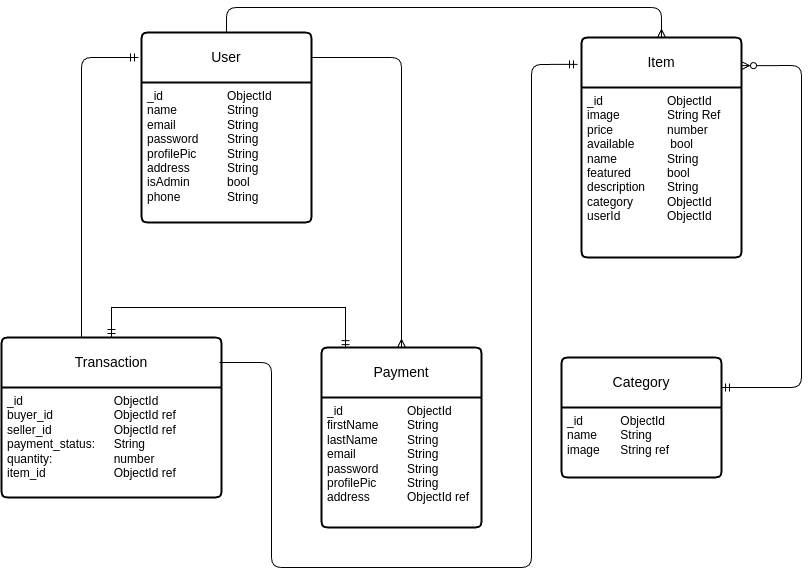
\includegraphics[scale=0.5]{../images/er.png}
    \caption{Entity-Relationship Diagram of ePurano}%
    \label{fig:er_diagram}
\end{figure}

The provided diagram is an Entity-Relationship (ER) diagram that depicts the relationships between various entities in the ePurano application. Here's a detailed explanation of each entity and their relationships:

\begin{enumerate}
    \item \textbf{User}
    \begin{itemize}
        \item The User entity represents individuals who use the ePurano platform to buy or sell secondhand items. Each user has a unique identifier userId, and other attributes such as name, email, password and profileImage
        \item A User can create multiple Items, meaning they can list several products for sale on the platform.
        \item A User can also be involved in multiple Transactions, either as a buyer or a seller, reflecting their activity within the marketplace.
    \end{itemize}

    \item \textbf{Item}
    \begin{itemize}
        \item The Item entity represents the secondhand goods listed for sale on ePurano. Each item has a unique identifier itemId and attributes such as title, description, price, and image.
        \item An Item is associated with one User, who is the seller listing the product. This is referenced by the userId foreign key.
        \item An Item belongs to one Category, linking it to a broader classification within the marketplace through the categoryId foreign key.
        \item An Item can be involved in multiple Transactions, indicating that it can be purchased multiple times by different users or repeatedly by the same user.
    \end{itemize}

    \item \textbf{Category}
    \begin{itemize}
        \item The Category entity represents the classification of Items within the ePurano marketplace. Each category has a unique identifier categoryId and a name attribute.
        \item A Category can have multiple Items, indicating that several products can belong to the same classification.
    \end{itemize}
    \item \textbf{Transaction}
    \begin{itemize}
        \item The Transaction entity represents the exchange of an Item between a buyer and a seller. Each transaction has a unique identifier transactionId.
        \item A Transaction involves one Item, linked through the itemId as a foreign key.
        \item A Transaction involves one Payment, indicating the financial transaction associated with the exchange. This is represented by the paymentId foreign key.
    \end{itemize}
    
    \item \textbf{Payment}
    \begin{itemize}
        \item The Payment entity represents the financial transaction for a purchase on ePurano. Each payment has a unique identifier paymentId and attributes such as amount, paymentDate, and user details.
        \item A Payment is associated with one Transaction, indicating that each financial transaction corresponds to a single exchange of goods.
    \end{itemize}
    
\end{enumerate}
\newpage

\section{Dataflow Diagram}
\begin{figure}[ht]
    \centering
    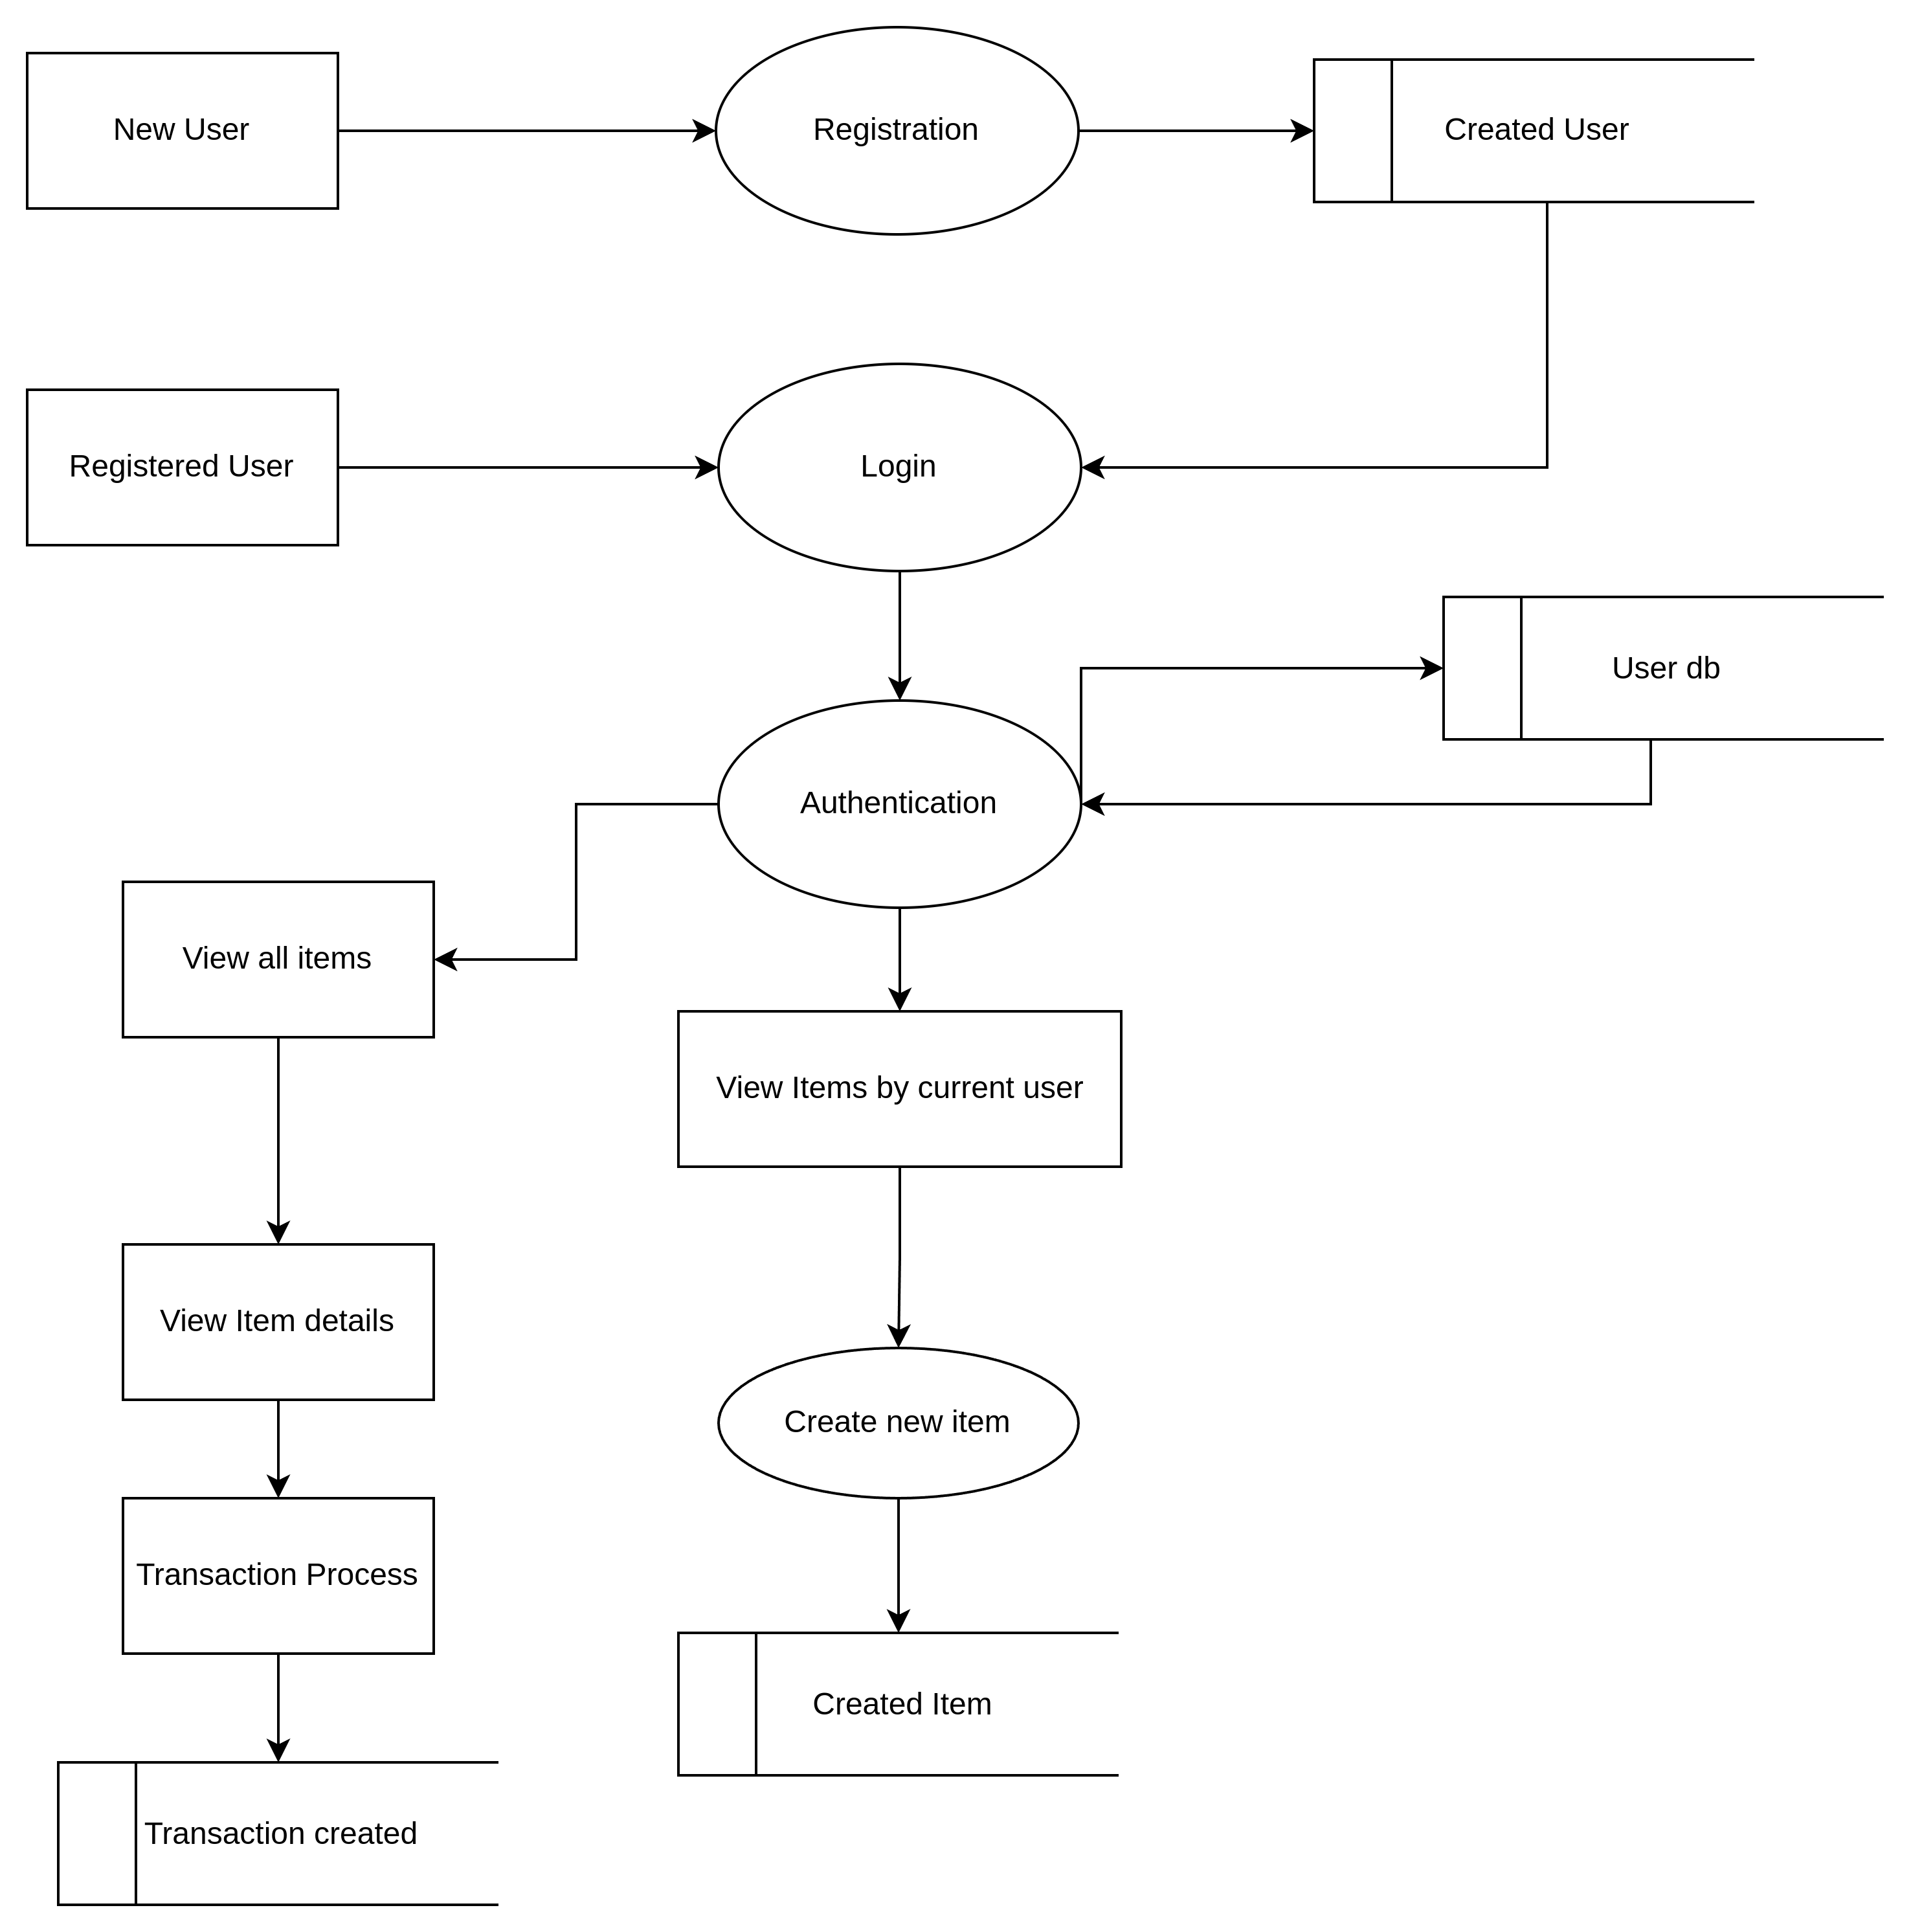
\includegraphics[scale=0.15]{../images/dataflow.png}
    \caption{Dataflow Diagram of ePurano}%
    \label{fig:data_flow_diagram}
\end{figure}

The Data Flow diagram shows a high-level overview of how a data flows inside the system where a new user register or an already registered user log in. The new user goes through the registration process and verification process and after that the user record is saved to the database. The existing user log in by going through authentication process. After logging in, they can view different items and can create their own. The Payment is done by cash on delivery or using the Khalti online payment gateway.

\newpage
\section{State Diagram}

\begin{figure}[ht]
    \centering
    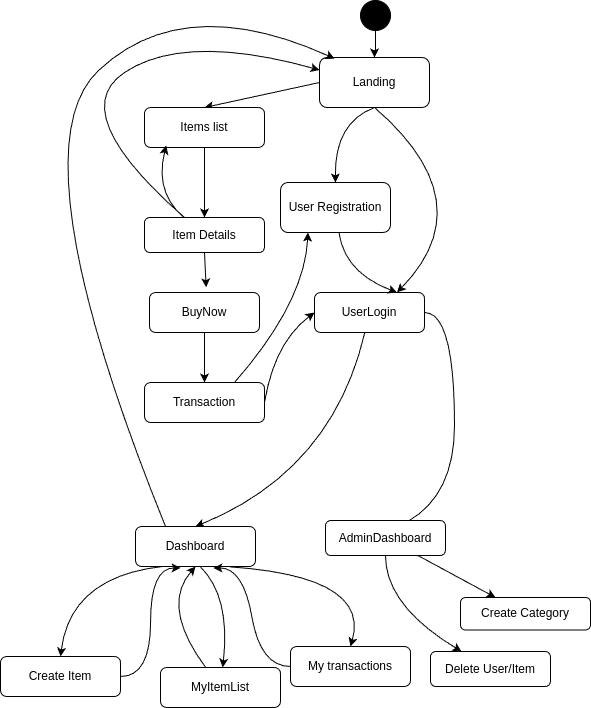
\includegraphics[scale=0.5]{../images/state.png}
    \caption{State Diagram of ePurano}%
    \label{fig:state_diagram}
\end{figure}
The state diagram for the ePurano application illustrates the various states the system can be in and the transitions between these states based on user actions. 

\newpage

\section{Use Case Diagram}
\begin{figure}[ht]
    \centering
    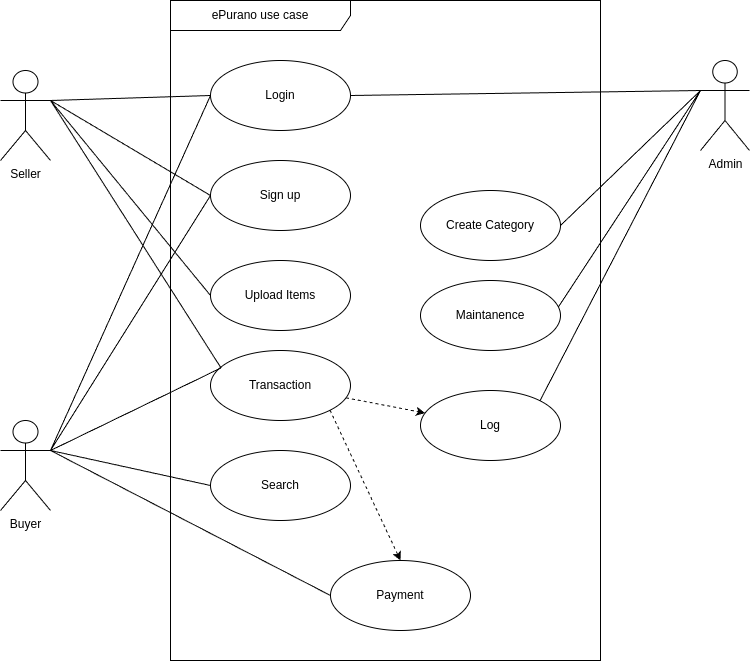
\includegraphics[scale=0.5]{../images/usecase.png}
    \caption{Use Case Diagram of ePurano}%
    \label{fig:usecase_diagram}
\end{figure}

The use case diagram for the ePurano application illustrates the different interactions between users (both regular users and admins) and the system. Here's a detailed description of each use case and the associated actors:

\begin{enumerate}
    \item \textbf{Login}
    \begin{description}
        \item[Actor] User, Admin 
        \item[Description] Both users and admins can log in to the system to access their respective dashboards and functionalities.
    \end{description}
    \item \textbf{Register}
    \begin{description}
        \item[Actor] User
        \item[Description] New users can register an account on the platform to start buying and selling secondhand items.
    \end{description}
    \item \textbf{Create Item}
    \begin{description}
        \item[Actor] User
        \item[Description] Registered users can upload details and images of the items they wish to sell.
    \end{description}
    \item \textbf{Transaction}
    \begin{description}
        \item[Actor] User
        \item[Description] Users can complete transactions for purchasing items listed on the platform.
    \end{description}
    \item \textbf{Create Category}
    \begin{description}
        \item[Actor] Admin
        \item[Description] Admins can create new categories for items, helping to organize listings and improve searchability.
    \end{description}
\end{enumerate}